\chapter{Instrukcja wdrożeniowa}

\section{Wymagane narzędzia}
Aplikacja w formie minimalnego środowiska uruchomieniowego stworzona w pracy dyplomowej dostępną jest na repozytorium GitHub pod poniższym linkiem: \newline
 \textbf{https://github.com/Maurycjo/Praca-dyplomowa/tree/release}
\newline

Do uruchomienia aplikacji niezbędne jest posiadanie następujących narzędzi \ref{tab:zestawienie_narzędzi}: 
\begin{itemize}
	\item Java 17
	\item Node v18.17.0
	\item SQL Server Management Studio
	\item SQL Server 
\end{itemize}

SSMS i SQL Server dostępne są na stronie Microsoftu.


\section{Konfigurowanie środowiska}

\begin{figure}[b]
		\centering
    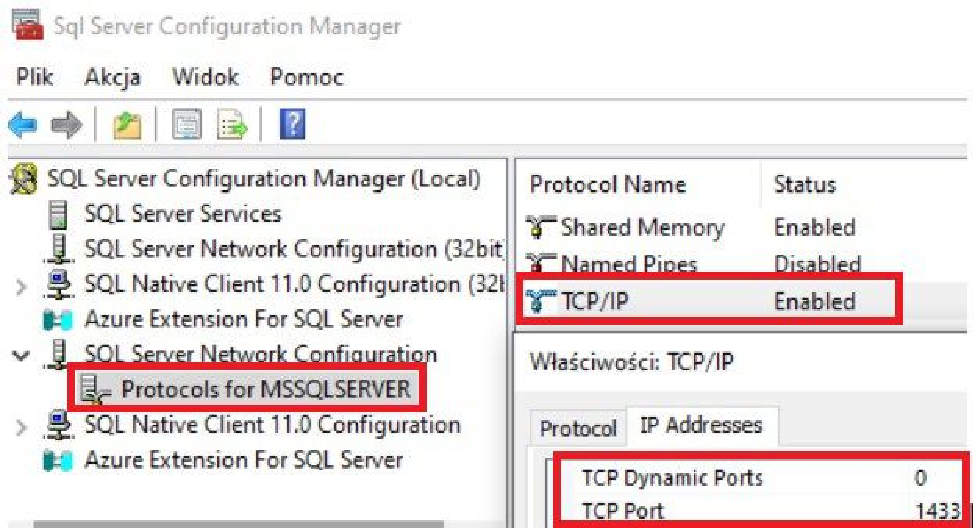
\includegraphics[width=0.6\linewidth]{rysA/tcpip.pdf}
    \caption{Konfiguracja TCP/IP}
    \label{tcpip:label}
\end{figure}

Wykorzystując narzędzie SQL Server Configuration Manager(instalowane z SQL Server) należy odblokować \textbf{TCP/IP} dla protokołu \textbf{MSSQLSERVER}. W właściwościach protokołu \textbf{TCP/IP}należy ustawić: TCP Dynamics Ports: \textbf{0} i pozostawić domyślny TCP Port: \textbf{1433}. Pokazano to na rysunku \ref{tcpip:label}.


\begin{figure}[htb]
  \centering
	\begin{tabular}{@{}lll@{}}
	a) & b) & c) \\
  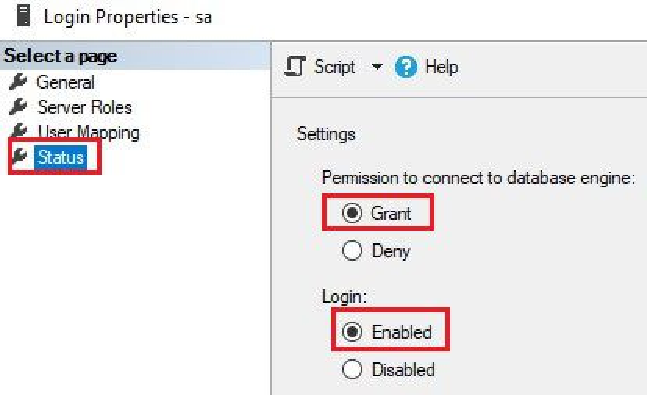
\includegraphics[width=0.300\textwidth]{rysA/status.pdf} & 
	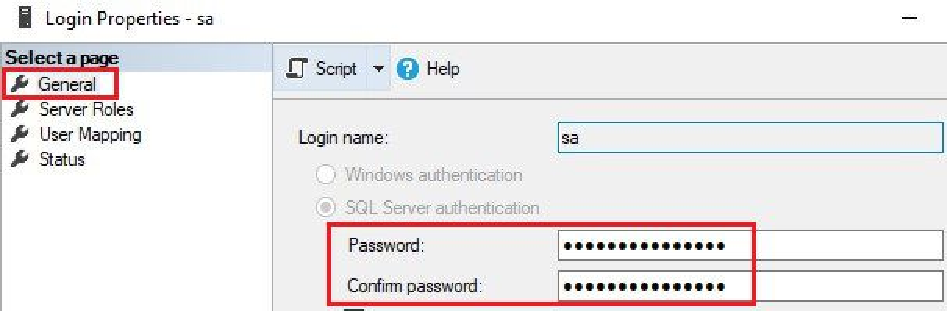
\includegraphics[width=0.333\textwidth]{rysA/general.pdf} &
	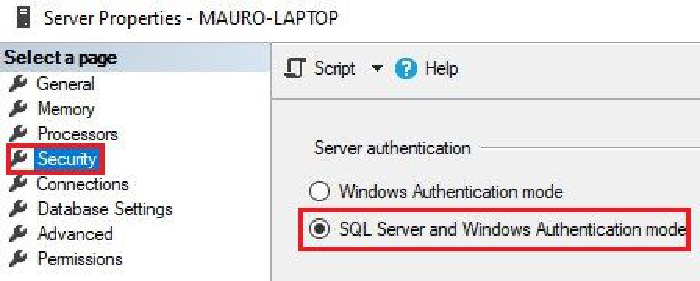
\includegraphics[width=0.320\textwidth]{rysA/enable.pdf}
	\end{tabular}
  \caption{Konfiguracja konta a) uprawnienia, b) zmiana hasła, c)typ uwierzytelniania }
  \label{sa:label}
\end{figure}

\newpage
\textbf{Konfiguracja konta:}
\begin{itemize}
\item należy zalogować się połączyć z serwerem SQL z użyciem Windows Authentication,
\item w folderze Security/Logins dla użytkownika "`\textbf{sa}"' należy ustawić mozliwość logowania oraz dać możliwość łączenia się z bazą danych co pokazano na rysunku \ref{sa:label}a
\item dla użytkownika "`sa"' należy również zmienić hasło na: "`\textbf{maurycy123}"' co pokazano na rysunku \ref{sa:label}b,
\item dla właściwości serwera w zakładce "`\emph{security}"' należy ustawić Server authentication na SQL Server and Windows Authentication co pokazano na rysunku \ref{sa:label}c, 
\item należy zrestartować komputer by ustawienia zadziałały,
\item teraz można logować się w SSMS przy użyciu SQL Server Authentication
\end{itemize}

Następnym krokiem jest importowanie bazy danych. Skrypt zawierający model i dane znajduje się w pobranym z repozytorium folderze Sql. Należy w SSMS utworzyć bazę danych o~nazwie "`\textbf{\texttt{DeviceLotery}}"'. Następnie klikając prawym przyciskiem myszy na utworzoną bazę danych należy wybrać opcje "`\textbf{\emph{New Query}}"', przekopiować skrypt i kliknąć przycisk prawy przycisk myszy z opcją \textbf{\emph{execute}}.

\textbf{Uruchamianie aplikacji serwerowej:}
Należy z linii komend uruchomić komendę: \mbox{\texttt{java -jar ComputerManagementTool-0.0.1-SNAPSHOT.jar}}

\textbf{Uruchamianie aplikacji klienckiej:}
Należy zainstalować pakiet \texttt{serve} z wykorzystaniem komendy: \textbf{\texttt{npm install -g serve}}. Następnie należy wykonać polecenie \textbf{\texttt{serve -s build}}

\textbf{Logowanie do aplikacji klienckiej:}
W systemie istnieją konta z różnymi uprawnieniami. Poniższa tabela \ref{tab:loginKlient} przedstawia loginy, hasła i role w systemie
 

\begin{table}[htb] \small
	\centering
\caption{Loginy i hasła aplikacji klienckiej}
\label{tab:loginKlient}
\begin{tabularx}{0.5\linewidth}{|X|X|X|}
		\hline
    Login & Hasło & Rola \\
		\hline
    admin & admin & Administrator\\
    \hline
    mniewczas & maurycy & Pracownik \\
    \hline
    jkowalski & maurycy &  Pracownik \\
    \hline
    lewy & maurycy & Pracownik \\
    \hline
\end{tabularx}
\end{table}




















